\documentclass{standalone} 
\usepackage{tikz}

\begin{document}
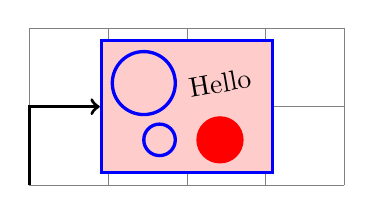
\begin{tikzpicture}
	\draw[help lines] (0,0) grid (4,2);
	% draw a matrix table
	\node [matrix,fill=red!20,draw=blue,very thick] (my matrix) at (2,1)
	% draw four elements, each in one of the cells
	{
		\draw (0,0) circle (4mm);   & \node[rotate=10] {Hello}; \\
		\draw (0.2,0) circle (2mm); & \fill[red] (0,0) circle (3mm); \\
	};
	% draw the arrow from the origin
	\draw [very thick,->] (0,0) |- (my matrix.west);
\end{tikzpicture}
\end{document}